% ============================================================
% PHẦN 5 — KẾT QUẢ THỰC NGHIỆM
% Người phụ trách: mỗi thành viên tự viết cho mô hình của mình
% ============================================================

\section{Kết quả thực nghiệm}
\label{sec:results}

\textit{Phần này do từng thành viên tự hoàn thiện cho mô hình của mình (Mục~\ref{subsec:res_maskrcnn}
đến \ref{subsec:res_mask2former}), sau đó cả nhóm tổng hợp bảng so sánh chung
(Mục~\ref{subsec:comparison}). Phần tinh chỉnh RF-DETR chỉ mô tả phương pháp chọn cấu hình fine-tune, không xem như một thí nghiệm tuning tự động riêng.}

% ----------------------------------------
\subsection{Mask R-CNN --- \textit{Lê Xuân Trí}}
\label{subsec:res_maskrcnn}

\subsubsection{Biểu đồ quá trình học (Learning Curves)}
\textit{[TODO --- Lê Xuân Trí: Chèn biểu đồ Loss và mAP@50 trên Train/Val theo epoch cho cả tập Rice và Coffee (4 biểu đồ). Nhận xét: mô hình có hội tụ không? Có dao động mạnh? Dấu hiệu overfitting/underfitting?]}

\subsubsection{Đánh giá trên tập Test}
\textit{[TODO --- Lê Xuân Trí: Điền bảng kết quả mAP@50, mAP@50:95, mIoU, Dice, inference time, model size cho cả Rice và Coffee.]}

\subsubsection{Confusion Matrix}
\textit{[TODO --- Lê Xuân Trí: Chèn confusion matrix per-class của Mask R-CNN trên tập Test (Rice và Coffee). Nhận xét lớp nào bị nhầm nhiều nhất.]}

% ----------------------------------------
\subsection{YOLO26-seg --- \textit{Nguyễn Hồ Anh Tuấn}}
\label{subsec:res_yolo}

\subsubsection{Biểu đồ quá trình học (Learning Curves)}
\textit{[TODO --- Nguyễn Hồ Anh Tuấn: Chèn biểu đồ Loss và mAP@50 trên Train/Val theo epoch cho cả Rice và Coffee. Nhận xét hội tụ.]}

\subsubsection{Đánh giá trên tập Test}
\textit{[TODO --- Nguyễn Hồ Anh Tuấn: Điền bảng kết quả đầy đủ.]}

\subsubsection{Confusion Matrix}
\textit{[TODO --- Nguyễn Hồ Anh Tuấn: Chèn confusion matrix và nhận xét.]}

% ----------------------------------------
\subsection{RF-DETR --- \textit{Tống Thanh Phúc}}
\label{subsec:res_rfdetr}

\subsubsection{Biểu đồ quá trình học (Learning Curves)}
Sau khi huấn luyện, notebook xuất các file:

\begin{verbatim}
report/data/rfdetr/coffee_training_log.csv
report/img/rfdetr/coffee_training_curve.png
report/data/rfdetr/rice_training_log.csv
report/img/rfdetr/rice_training_curve.png
\end{verbatim}

Các file này được lấy từ output đã lưu của hai notebook \texttt{train-eva-coffee.ipynb} và \texttt{train-eva-rice.ipynb}, sau đó được đổi tên và đặt lại trong thư mục \texttt{report/} để báo cáo có thể tham chiếu trực tiếp. File CSV lưu log/metric theo quá trình train, còn file PNG là biểu đồ learning curve đã export.

\begin{figure}[H]
    \centering
    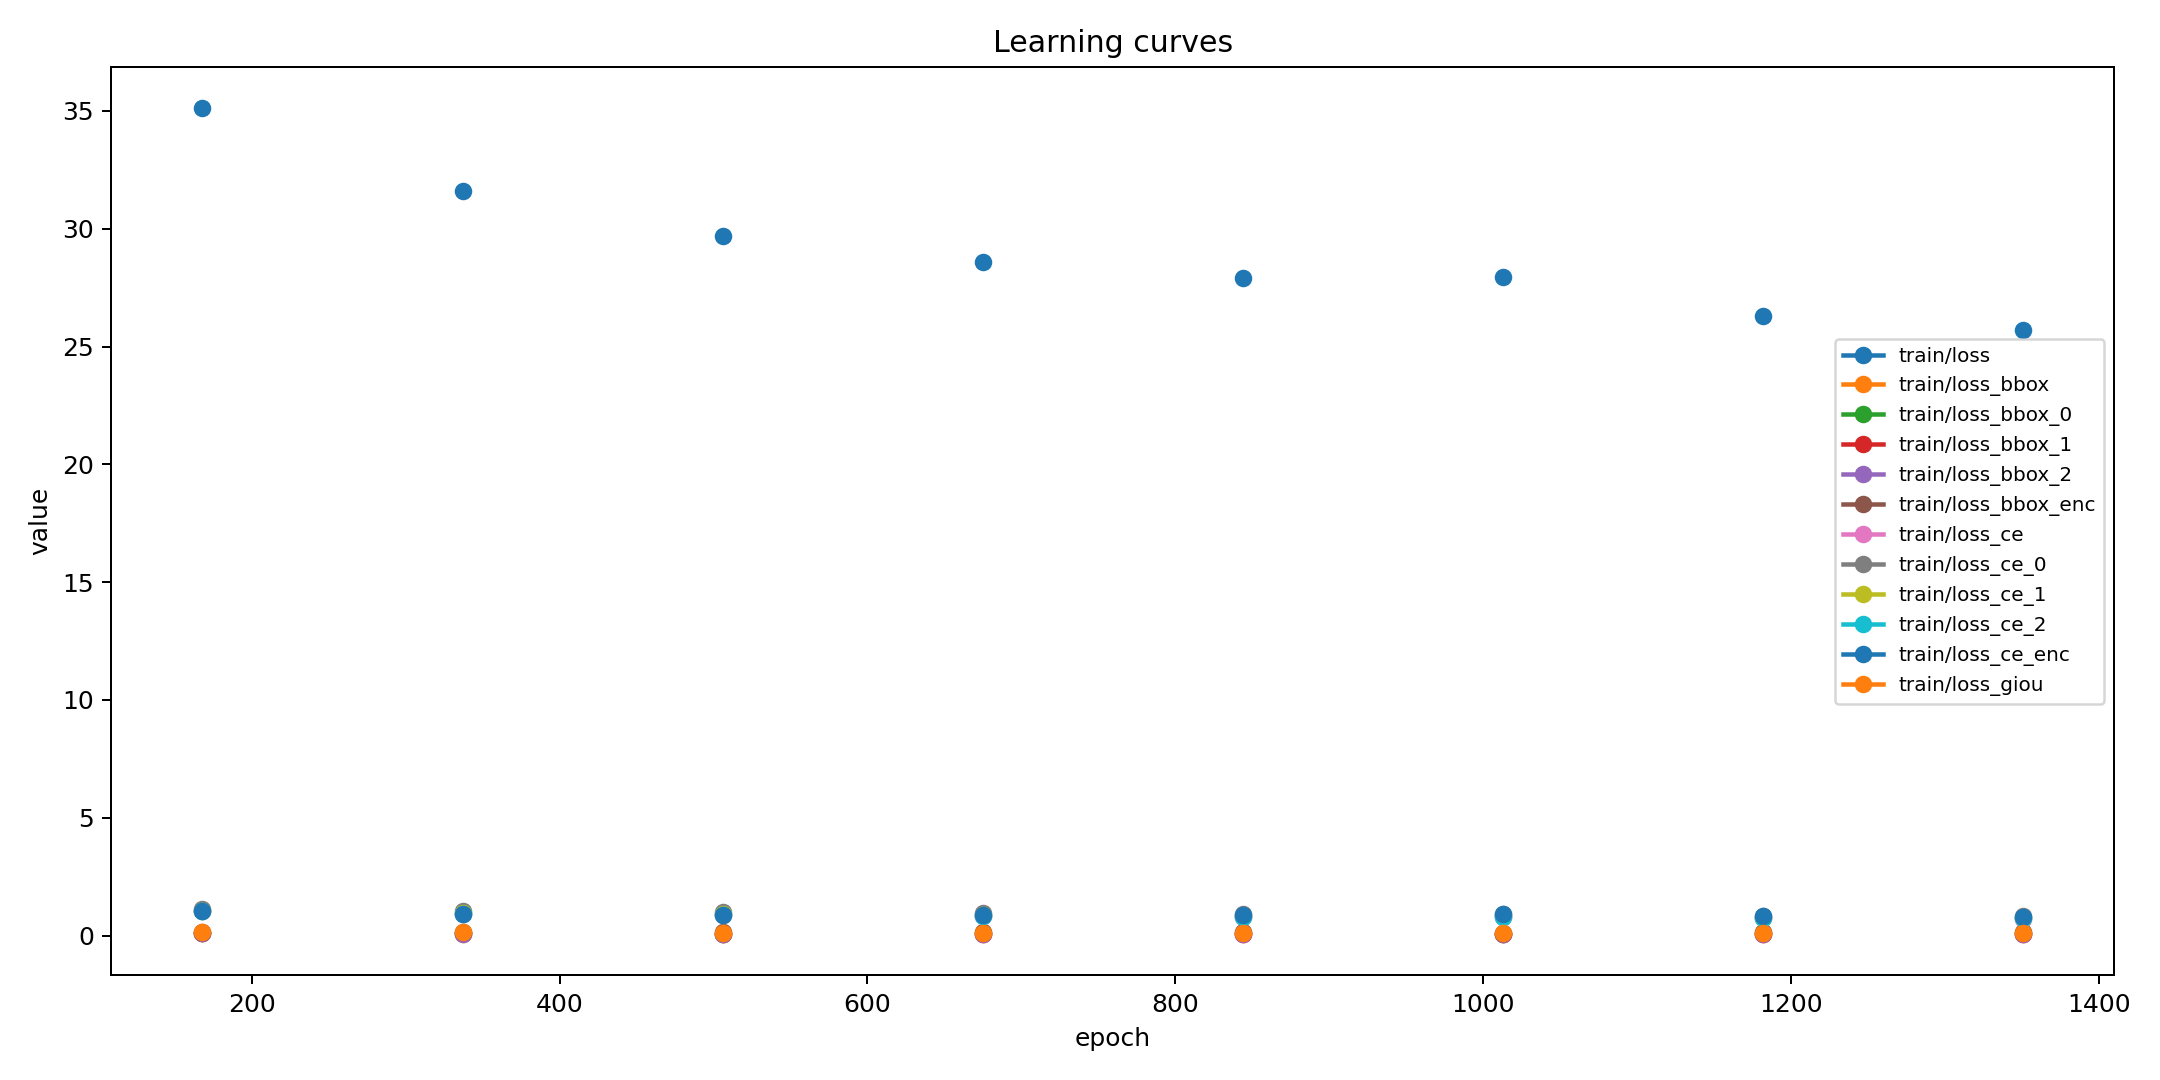
\includegraphics[width=0.92\textwidth]{img/rfdetr/coffee_training_curve.png}
    \caption{Biểu đồ kết quả huấn luyện RF-DETR trên tập coffee}
    \label{fig:rfdetr_coffee_curve}
\end{figure}

\begin{figure}[H]
    \centering
    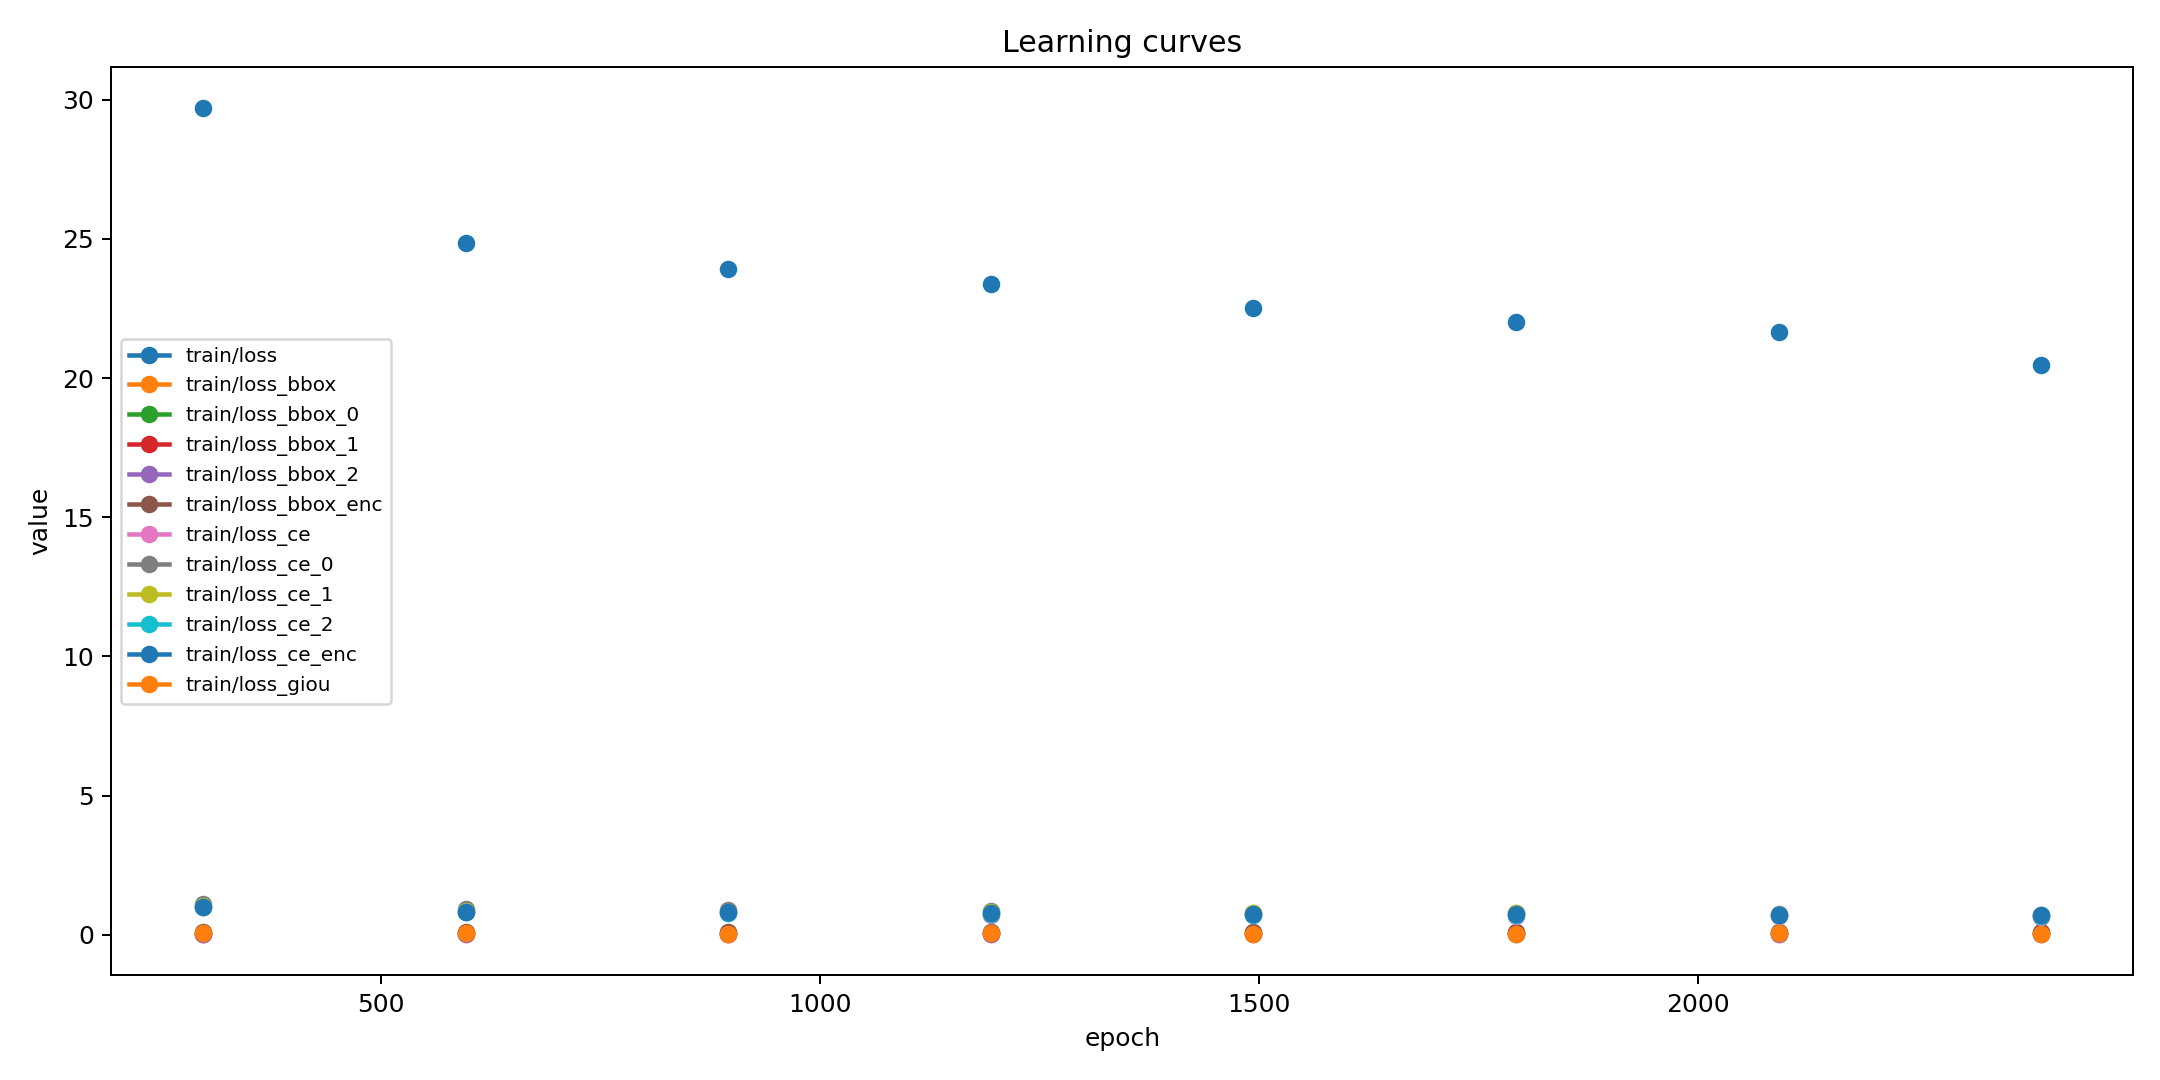
\includegraphics[width=0.92\textwidth]{img/rfdetr/rice_training_curve.png}
    \caption{Biểu đồ kết quả huấn luyện RF-DETR trên tập rice}
    \label{fig:rfdetr_rice_curve}
\end{figure}

Nhìn chung, notebook dùng best checkpoint thay vì model ở epoch cuối để evaluate. Điều này giúp giảm rủi ro chọn checkpoint bị dao động ở cuối quá trình train. Trên validation, coffee đạt \texttt{val/segm\_mAP\_50} cao nhất khoảng $0.9207$ ở epoch cuối được log, trong khi rice đạt khoảng $0.7592$. Đường cong rice dao động hơn coffee, phù hợp với nhận xét rằng tập rice có nhiều annotation và cấu trúc bệnh phức tạp hơn.

\subsubsection{Đánh giá trên tập Test}
Kết quả dưới đây được lấy từ output đã lưu trong hai notebook \texttt{train-eva-coffee.ipynb} và \texttt{train-eva-rice.ipynb}. Cả hai mô hình được evaluate trên split \texttt{test}.

\begin{table}[H]
    \caption{Kết quả RF-DETR trên tập Test}
    \centering
    \begin{tabular}{lrrrrrrr}
        \toprule
        \textbf{Domain} & \textbf{Test images} & \textbf{mAP50 bbox} & \textbf{mAP50:95 bbox} & \textbf{mAP50 segm} & \textbf{mAP50:95 segm} & \textbf{mIoU} & \textbf{Dice} \\
        \midrule
        Coffee & 576 & 0.820 & 0.598 & 0.842835 & 0.825083 & 0.857505 & 0.871758 \\
        Rice   & 514 & 0.736 & 0.718 & 0.703828 & 0.687440 & 0.813240 & 0.830791 \\
        \bottomrule
    \end{tabular}
    \label{tab:rfdetr_test_results}
\end{table}

Vì bài toán chính là segmentation, hai chỉ số quan trọng nhất là \textbf{mAP50 segm} và \textbf{mAP50:95 segm}. Trên coffee, RF-DETR đạt mAP50:95 segmentation cao hơn rice. Điều này cho thấy mô hình học mask trên coffee ổn định hơn trong lần chạy hiện tại. Rice có nhiều ảnh chứa nhiều annotation và hình thái bệnh phức tạp hơn, nên kết quả mAP segmentation thấp hơn nhưng vẫn đạt Dice và mIoU khá tốt.

Thời gian suy luận trung bình:

\begin{itemize}
    \item Coffee: 70.306 ms/ảnh.
    \item Rice: 198.306 ms/ảnh.
\end{itemize}

\subsubsection{Confusion Matrix}
Notebook xuất confusion matrix cho từng domain tại:

\begin{verbatim}
report/img/rfdetr/coffee_confusion_matrix.png
report/img/rfdetr/rice_confusion_matrix.png
\end{verbatim}

Confusion matrix được xây dựng bằng cách match prediction với ground truth trên test set theo ngưỡng IoU $0.5$. Ngoài các lớp bệnh, ma trận có thêm hai nhóm hỗ trợ phân tích lỗi:

\begin{itemize}
    \item \texttt{\_\_missed\_\_}: ground truth không được mô hình phát hiện đúng.
    \item \texttt{\_\_background\_\_}: prediction dư hoặc không khớp ground truth.
\end{itemize}

\begin{figure}[H]
    \centering
    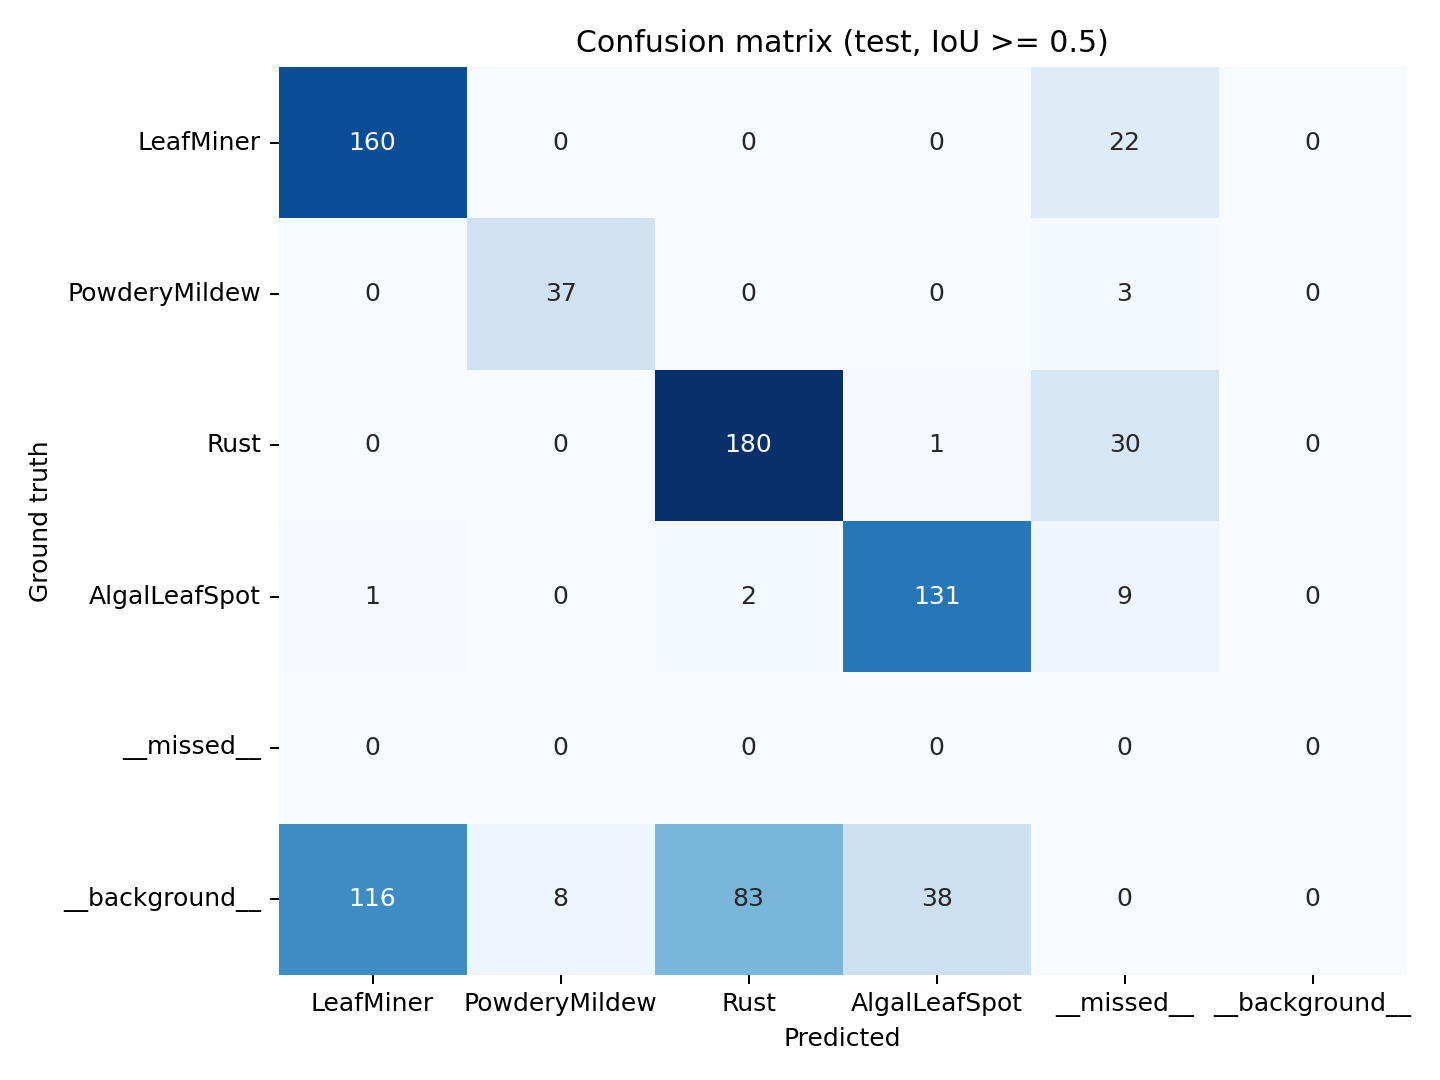
\includegraphics[width=0.82\textwidth]{img/rfdetr/coffee_confusion_matrix.png}
    \caption{Confusion matrix RF-DETR trên tập test coffee}
    \label{fig:rfdetr_coffee_cm}
\end{figure}

\begin{figure}[H]
    \centering
    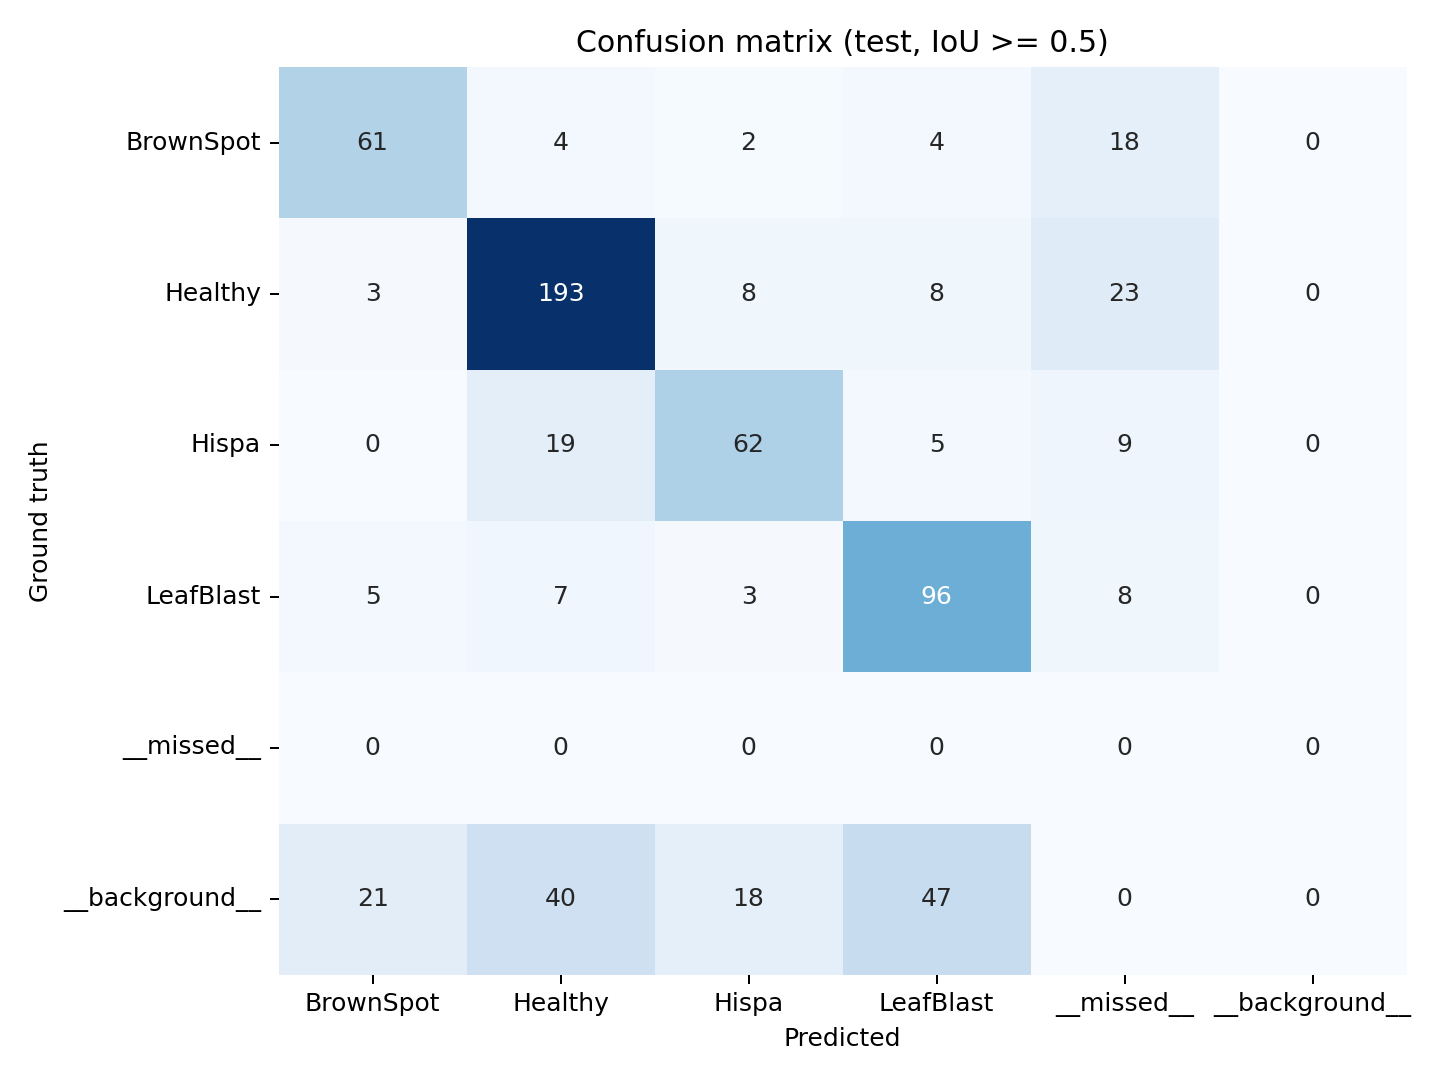
\includegraphics[width=0.82\textwidth]{img/rfdetr/rice_confusion_matrix.png}
    \caption{Confusion matrix RF-DETR trên tập test rice}
    \label{fig:rfdetr_rice_cm}
\end{figure}

Bảng dưới đây tóm tắt precision, recall và F1 theo lớp từ các file \texttt{coffee\_classification\_metrics.csv} và \texttt{rice\_classification\_metrics.csv} trong \texttt{report/data/rfdetr/}.

\begin{table}[H]
    \caption{Kết quả phân loại theo lớp của RF-DETR trên test set}
    \centering
    \begin{tabular}{llrrrrrr}
        \toprule
        \textbf{Domain} & \textbf{Lớp} & \textbf{TP} & \textbf{FP} & \textbf{FN} & \textbf{Precision} & \textbf{Recall} & \textbf{F1} \\
        \midrule
        Coffee & LeafMiner      & 160 & 117 & 22 & 0.578 & 0.879 & 0.697 \\
        Coffee & PowderyMildew  & 37  & 8   & 3  & 0.822 & 0.925 & 0.871 \\
        Coffee & Rust           & 180 & 85  & 31 & 0.679 & 0.853 & 0.756 \\
        Coffee & AlgalLeafSpot  & 131 & 39  & 12 & 0.771 & 0.916 & 0.837 \\
        Rice   & BrownSpot      & 61  & 29  & 28 & 0.678 & 0.685 & 0.682 \\
        Rice   & Healthy        & 193 & 70  & 42 & 0.734 & 0.821 & 0.775 \\
        Rice   & Hispa          & 62  & 31  & 33 & 0.667 & 0.653 & 0.660 \\
        Rice   & LeafBlast      & 96  & 64  & 23 & 0.600 & 0.807 & 0.688 \\
        \bottomrule
    \end{tabular}
    \label{tab:rfdetr_class_metrics}
\end{table}

Với coffee, RF-DETR nhận diện tốt nhất các lớp \texttt{PowderyMildew} và \texttt{AlgalLeafSpot}, lần lượt đạt F1 khoảng $0.871$ và $0.837$. Lớp \texttt{LeafMiner} có recall cao ($0.879$) nhưng precision thấp hơn ($0.578$), nguyên nhân chính là nhiều prediction dư bị gom vào nhóm \texttt{\_\_background\_\_}. Lớp \texttt{Rust} cũng có số false positive tương đối lớn, nhưng vẫn giữ F1 khoảng $0.756$.

Với rice, lớp \texttt{Healthy} có F1 cao nhất ($0.775$), còn \texttt{Hispa} thấp nhất ($0.660$). Confusion matrix cho thấy \texttt{Hispa} dễ bị nhầm sang \texttt{Healthy}, trong khi \texttt{LeafBlast} có recall tốt nhưng precision thấp hơn do nhiều prediction dư. Như vậy phần còn yếu của RF-DETR trên rice không chỉ nằm ở bỏ sót đối tượng mà còn ở false positive trên nền và nhầm giữa các lớp có biểu hiện thị giác gần nhau.

% ----------------------------------------
\subsection{MobileSAM --- \textit{Đàm Tiến Đạt}}
\label{subsec:res_mobilesam}

\subsubsection{Biểu đồ quá trình học (Learning Curves)}
\textit{[TODO --- Đàm Tiến Đạt: Chèn biểu đồ Loss và mIoU trên Train/Val theo epoch cho cả Rice và Coffee. Nhận xét hội tụ.]}

\subsubsection{Đánh giá trên tập Test}
\textit{[TODO --- Đàm Tiến Đạt: Điền bảng kết quả đầy đủ.]}

\subsubsection{Confusion Matrix}
\textit{[TODO --- Đàm Tiến Đạt: Chèn confusion matrix và nhận xét.]}

% ----------------------------------------
\subsection{Mask2Former --- \textit{Dương Tuấn Anh}}
\label{subsec:res_mask2former}

\subsubsection{Biểu đồ quá trình học (Learning Curves)}
\textit{[TODO --- Dương Tuấn Anh: Chèn biểu đồ Loss và mAP@50 trên Train/Val theo epoch cho cả Rice và Coffee. Nhận xét hội tụ.]}

\subsubsection{Đánh giá trên tập Test}
\textit{[TODO --- Dương Tuấn Anh: Điền bảng kết quả đầy đủ.]}

\subsubsection{Confusion Matrix}
\textit{[TODO --- Dương Tuấn Anh: Chèn confusion matrix và nhận xét.]}

% ----------------------------------------
\subsection{Bảng so sánh tổng hợp (Phase 3)}
\label{subsec:comparison}

\textit{[TODO --- Cả nhóm tổng hợp sau khi 5 thành viên hoàn thành. Tô đậm hàng của mô hình được chọn làm best model.]}

\begin{table}[H]
    \caption{Kết quả đánh giá 5 mô hình trên tập Test --- Rice dataset}
    \centering
    \begin{tabular}{lrrrrrr}
        \toprule
        \textbf{Mô hình} & \textbf{mAP@50} & \textbf{mAP@50:95} & \textbf{mIoU} & \textbf{Dice} & \textbf{Infer (ms)} & \textbf{Size (MB)} \\
        \midrule
        Mask R-CNN    & --- & --- & --- & --- & --- & --- \\
        YOLO26-seg    & --- & --- & --- & --- & --- & --- \\
        RF-DETR       & 0.704 & 0.687 & 0.813 & 0.831 & 198.306 & 133 \\
        MobileSAM     & --- & --- & --- & --- & --- & --- \\
        Mask2Former   & --- & --- & --- & --- & --- & --- \\
        \bottomrule
    \end{tabular}
    \label{tab:results_rice}
\end{table}

\begin{table}[H]
    \caption{Kết quả đánh giá 5 mô hình trên tập Test --- Coffee dataset}
    \centering
    \begin{tabular}{lrrrrrr}
        \toprule
        \textbf{Mô hình} & \textbf{mAP@50} & \textbf{mAP@50:95} & \textbf{mIoU} & \textbf{Dice} & \textbf{Infer (ms)} & \textbf{Size (MB)} \\
        \midrule
        Mask R-CNN    & --- & --- & --- & --- & --- & --- \\
        YOLO26-seg    & --- & --- & --- & --- & --- & --- \\
        RF-DETR       & 0.843 & 0.825 & 0.858 & 0.872 & 70.306 & 133 \\
        MobileSAM     & --- & --- & --- & --- & --- & --- \\
        Mask2Former   & --- & --- & --- & --- & --- & --- \\
        \bottomrule
    \end{tabular}
    \label{tab:results_coffee}
\end{table}

% ----------------------------------------
\subsection{Phương pháp tinh chỉnh cấu hình RF-DETR}
\label{subsec:tuning_results}

Trong phạm vi notebook hiện tại, nhóm không chạy RayTune ASHA, grid search hay một quá trình tuning tự động nhiều thử nghiệm. Do đó báo cáo không trình bày bảng before/after tuning riêng. Phần tinh chỉnh chỉ được hiểu là phương pháp chọn cấu hình fine-tune phù hợp với tài nguyên Kaggle và đặc thù dữ liệu.

Cụ thể, nhóm giữ model size là \texttt{nano}, số epoch là $8$, learning rate là $1\times10^{-4}$ và encoder learning rate là $1.5\times10^{-4}$. Khác biệt chính giữa hai domain nằm ở batch size: coffee dùng batch size $4$, còn rice dùng batch size $2$ do ảnh và annotation phức tạp hơn, dễ tốn VRAM hơn. Gradient accumulation được đặt là $4$ để tăng batch hiệu dụng, đồng thời bật early stopping để tránh huấn luyện dư khi validation metric không còn cải thiện rõ.

Các artifact dùng để minh họa định tính gồm learning curve, confusion matrix và các file CSV metric. Những file này đã được chuyển vào báo cáo với tên thống nhất:

\begin{verbatim}
report/img/rfdetr/
report/data/rfdetr/
\end{verbatim}

Hiện tại artifact đã đủ để trình bày learning curve, confusion matrix và bảng metric cho cả hai domain. Kích thước mô hình trong bảng tổng hợp được ghi theo dung lượng best checkpoint, với cả coffee và rice đều khoảng $133$MB. Phần còn thiếu nếu muốn báo cáo đầy đủ hơn là file \texttt{config.json} và \texttt{class\_names.json} cho rice; class names hiện được suy ra từ các file CSV đã export.

